%
% fig-relief.tex
%
% (c) 2025 Prof Dr Andreas Müller
%
\begin{figure}
\centering
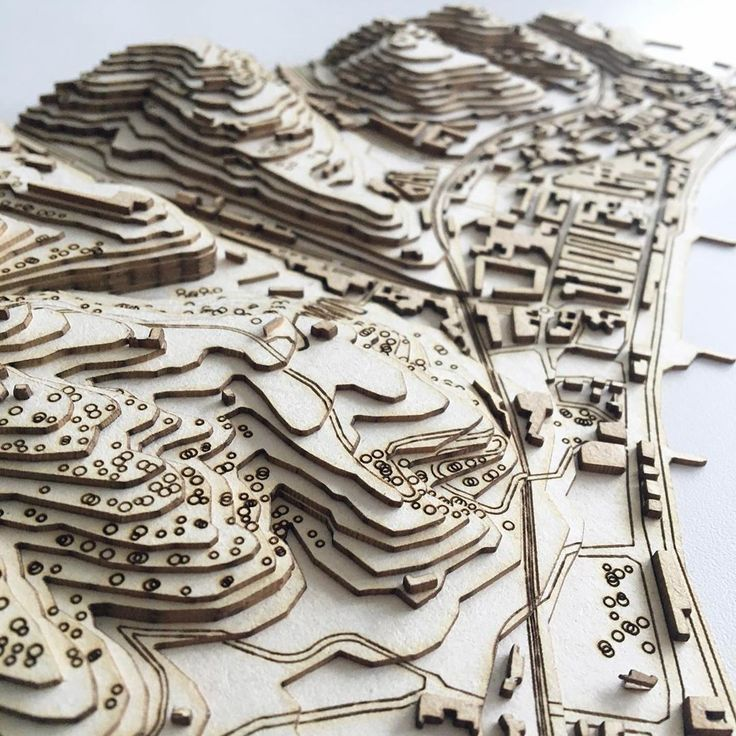
\includegraphics[width=0.7\textwidth]{chapters/120-topologie/images/relief.jpg}
\caption{Rekonstruktion einer Approximation der Topographie aus den
\index{Topographie}%
Höhenlinien mit Hilfe von Platten, die entlang der Höhenlinien ausgeschnitten
worden sind.
\label{buch:topologie:morse:fig:relief}}
\end{figure}
